\documentclass[9pt, aspectratio=169, handout]{beamer}

% +==================================================+
% |   ████████╗██╗  ██╗███████╗███╗   ███╗███████╗   |
% |   ╚══██╔══╝██║  ██║██╔════╝████╗ ████║██╔════╝   |
% |      ██║   ███████║█████╗  ██╔████╔██║█████╗     |
% |      ██║   ██╔══██║██╔══╝  ██║╚██╔╝██║██╔══╝     |
% |      ██║   ██║  ██║███████╗██║ ╚═╝ ██║███████╗   |
% |      ╚═╝   ╚═╝  ╚═╝╚══════╝╚═╝     ╚═╝╚══════╝   |
% +==================================================+

\useinnertheme{rectangles}
\useoutertheme{infolines}

\setbeamertemplate{footline}{%
    \leavevmode%
    \rule{\paperwidth}{0.1pt}\vskip0.2pt%
    \hbox{%
        \begin{beamercolorbox}[wd=.2\paperwidth, ht=2.25ex, dp=1ex, center]{author in head/foot}%
            \usebeamerfont{author in head/foot}\insertshortauthor
        \end{beamercolorbox}%
        \begin{beamercolorbox}[wd=.6\paperwidth, ht=2.25ex, dp=1ex, center]{title in head/foot}%
            \usebeamerfont{title in head/foot}\insertshorttitle
        \end{beamercolorbox}%
        \begin{beamercolorbox}[wd=.2\paperwidth, ht=2.25ex, dp=1ex, center]{date in head/foot}%
            \usebeamerfont{date in head/foot}\insertshortdate\hfill\insertframenumber{} / \inserttotalframenumber\hspace*{2ex}
        \end{beamercolorbox}%
    }%
    \vskip0pt%
}
% hrule under the frametitle, see:
% https://tex.stackexchange.com/questions/343517/beamer-full-width-hrule-below-frame-title
\setbeamertemplate{frametitle}{%
    \usebeamerfont{frametitle}\insertframetitle%
    \vphantom{g}%
    \par%
    \makebox[\linewidth][c]{%
        \rule[0.5\baselineskip]{\paperwidth}{0.4pt}%
    }%
}

% \beamertemplatenavigationsymbolsempty % remove navigation bar

\definecolor{grey80}{HTML}{CCCCCC}
\definecolor{grey90}{HTML}{E6E6E6}
\definecolor{grey95}{HTML}{F2F2F2}

\usepackage[svgnames, x11names]{xcolor}
\usecolortheme[named=DarkSlateGrey]{structure}
\setbeamercolor{background canvas}{bg=white}

\setbeamerfont{frametitle}{series=\bfseries}

\let\oldtiny\tiny
\let\oldscriptsize\scriptsize
\let\oldfootnotesize\footnotesize
\let\oldsmall\small
\let\oldnormalsize\normalsize
\let\oldlarge\large
\let\oldLarge\Large
\let\oldLARGE\LARGE
\let\oldhuge\huge
\let\oldHuge\Huge
\renewcommand*{\footnotesize}{\oldfootnotesize\scriptsize}
\renewcommand*{\normalsize}{\oldnormalsize\oldsmall}
\setbeamerfont{frametitle}{size=\oldnormalsize}

% +=================================+
% |   ██████╗ ██╗██████╗ ███████╗   |
% |   ██╔══██╗██║██╔══██╗██╔════╝   |
% |   ██████╔╝██║██████╔╝███████╗   |
% |   ██╔══██╗██║██╔══██╗╚════██║   |
% |   ██████╔╝██║██████╔╝███████║   |
% |   ╚═════╝ ╚═╝╚═════╝ ╚══════╝   |
% +=================================+

% \usepackage[style=nejm,backend=biber]{biblatex}
% \addbibresource{my.bib}
% \renewcommand*{\bibfont}{\footnotesize}

% +==========================================+
% |   ███╗   ███╗ █████╗ ████████╗██╗  ██╗   |
% |   ████╗ ████║██╔══██╗╚══██╔══╝██║  ██║   |
% |   ██╔████╔██║███████║   ██║   ███████║   |
% |   ██║╚██╔╝██║██╔══██║   ██║   ██╔══██║   |
% |   ██║ ╚═╝ ██║██║  ██║   ██║   ██║  ██║   |
% |   ╚═╝     ╚═╝╚═╝  ╚═╝   ╚═╝   ╚═╝  ╚═╝   |
% +==========================================+

\usepackage{amsmath,amssymb,amsfonts}
\usepackage{cancel}
\usepackage{braket}
\usepackage{bm}
\usepackage{siunitx}
\usepackage{feynmf}
\usepackage{cleveref}
\DeclareGraphicsRule{*}{mps}{*}{}

% +===================================================+
% |   ███████╗██╗ ██████╗ ██╗   ██╗██████╗ ███████╗   |
% |   ██╔════╝██║██╔════╝ ██║   ██║██╔══██╗██╔════╝   |
% |   █████╗  ██║██║  ███╗██║   ██║██████╔╝█████╗     |
% |   ██╔══╝  ██║██║   ██║██║   ██║██╔══██╗██╔══╝     |
% |   ██║     ██║╚██████╔╝╚██████╔╝██║  ██║███████╗   |
% |   ╚═╝     ╚═╝ ╚═════╝  ╚═════╝ ╚═╝  ╚═╝╚══════╝   |
% +===================================================+
\usepackage{subcaption}
\usepackage{makecell}
\usepackage{booktabs}

% +===========================================================+
% |    ██████╗██╗  ██╗██╗███╗   ██╗███████╗███████╗███████╗   |
% |   ██╔════╝██║  ██║██║████╗  ██║██╔════╝██╔════╝██╔════╝   |
% |   ██║     ███████║██║██╔██╗ ██║█████╗  ███████╗█████╗     |
% |   ██║     ██╔══██║██║██║╚██╗██║██╔══╝  ╚════██║██╔══╝     |
% |   ╚██████╗██║  ██║██║██║ ╚████║███████╗███████║███████╗   |
% |    ╚═════╝╚═╝  ╚═╝╚═╝╚═╝  ╚═══╝╚══════╝╚══════╝╚══════╝   |
% +===========================================================+

% \usepackage{xeCJK}
% \setCJKmainfont{PingFang SC}

% +====================================+
% |   ███╗   ███╗██╗███████╗ ██████╗   |
% |   ████╗ ████║██║██╔════╝██╔════╝   |
% |   ██╔████╔██║██║███████╗██║        |
% |   ██║╚██╔╝██║██║╚════██║██║        |
% |   ██║ ╚═╝ ██║██║███████║╚██████╗   |
% |   ╚═╝     ╚═╝╚═╝╚══════╝ ╚═════╝   |
% +====================================+

\usepackage{fontawesome5}
\usepackage{twemojis}
\newcommand{\myhl}[1]{\textcolor{DeepPink}{#1}}
\newcommand{\myhlb}[1]{\textcolor{Blue}{#1}}


\title{MAE 131A Discussion Sections\\ Week 1}
\author{Chuanjin Su}
\institute[UCLA MAE]{Mechanical and Aerospace Engineering Department\\
    University of California, Los Angeles}
\date{Oct 4, 2024}

\begin{document}

\begin{frame}
    \titlepage
\end{frame}

\begin{frame}{Problem 1}
    \begin{columns}
        \column{.3\textwidth}
        \begin{figure}
            \centering
            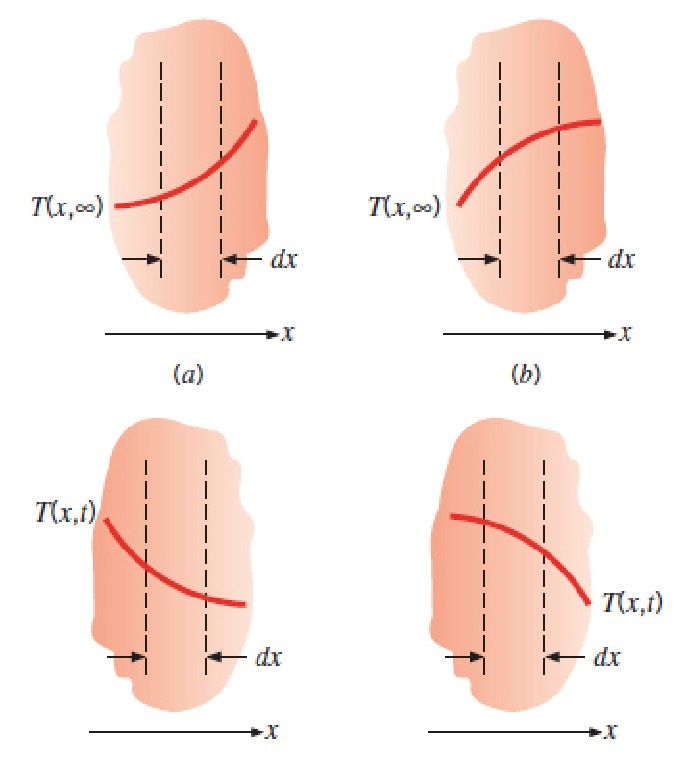
\includegraphics[width=\textwidth]{Figures/fig1.1.jpg}
        \end{figure}
        \column{.7\textwidth}
        Consider the temperature distribution associated with a $dx$ differential control volume within the one-dimensional plane walls shown on the left.
        \begin{itemize}
            \item[(a)] Steady-state conditions exist. Is thermal energy being generated within the differential control volume? If so, is the generation rate positive or negative?
            \item[(b)] Steady-state conditions exist as in part (a). Is the volumetric generation rate positive or negative within the differential control volume?
            \item[(c)] Steady-state conditions \myhl{do not} exist, and there is no volumetric thermal energy generation. Is the temperature of the material in the differential control volume increasing or decreasing with time?
            \item[(d)] Transient conditions exist as in part (c). Is the temperature increasing or decreasing with time?
        \end{itemize}
    \end{columns}
\end{frame}

\begin{frame}{Problem 1 Solution}
    \begin{columns}
        \column{.3\textwidth}
        \begin{figure}
            \centering
            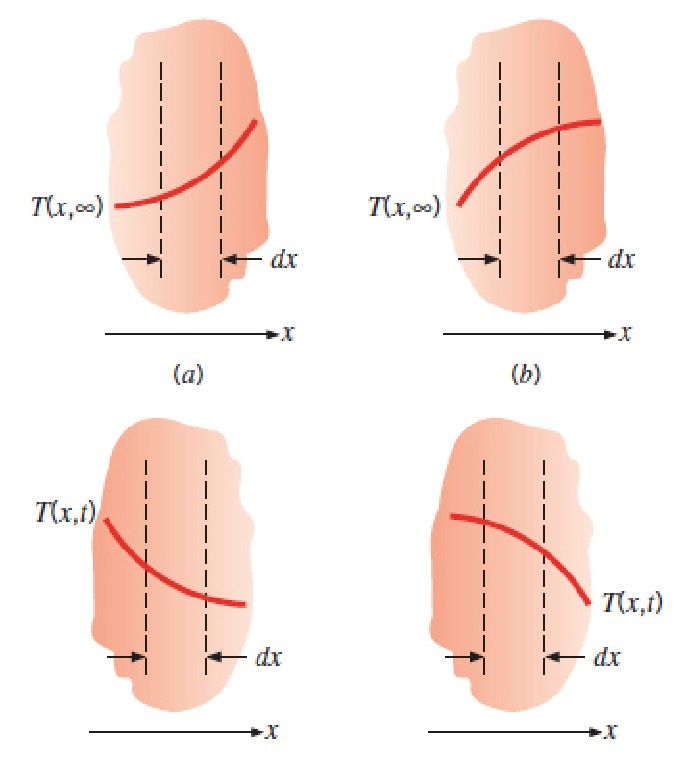
\includegraphics[width=\textwidth]{Figures/fig1.1.jpg}
        \end{figure}
        \column{.7\textwidth}
        \begin{itemize}
            \item[(a)] Steady-state conditions exist. Is thermal energy being generated within the differential control volume? If so, is the generation rate positive or negative?\par\pause
            \myhlb{Solution: } using the heat conduction equation: $\cancel{\rho c_v \frac{\partial T}{\partial t}} = k\frac{\partial^2 T}{\partial x^2} + \dot{Q}$, the sign of $\dot{Q}$ is in opposite to $\partial^2 T/\partial x^2$. Answer: Negative.\pause
            \item[(b)] Steady-state conditions exist as in part (a). Is the volumetric generation rate positive or negative within the differential control volume?\par\pause
            \myhlb{Solution: } Same as (a), but the sign of $\dot{Q}$ is positive.\pause
            \item[(c)] Steady-state conditions \myhl{do not} exist, and there is no volumetric thermal energy generation. Is the temperature of the material in the differential control volume increasing or decreasing with time?\par\pause
            \myhlb{Solution: } $\rho c_v \frac{\partial T}{\partial t} = k\frac{\partial^2 T}{\partial x^2} + \cancel{\dot{Q}}$. Answer: Increasing.\pause
            \item[(d)] Transient conditions exist as in part (c). Is the temperature increasing or decreasing with time?\par\pause
            \myhlb{Solution: } Same as (c). Answer: decreasing.
        \end{itemize}
    \end{columns}
\end{frame}

\begin{frame}{Problem 2 (3.18 in the book)}
    \begin{figure}
        \centering
        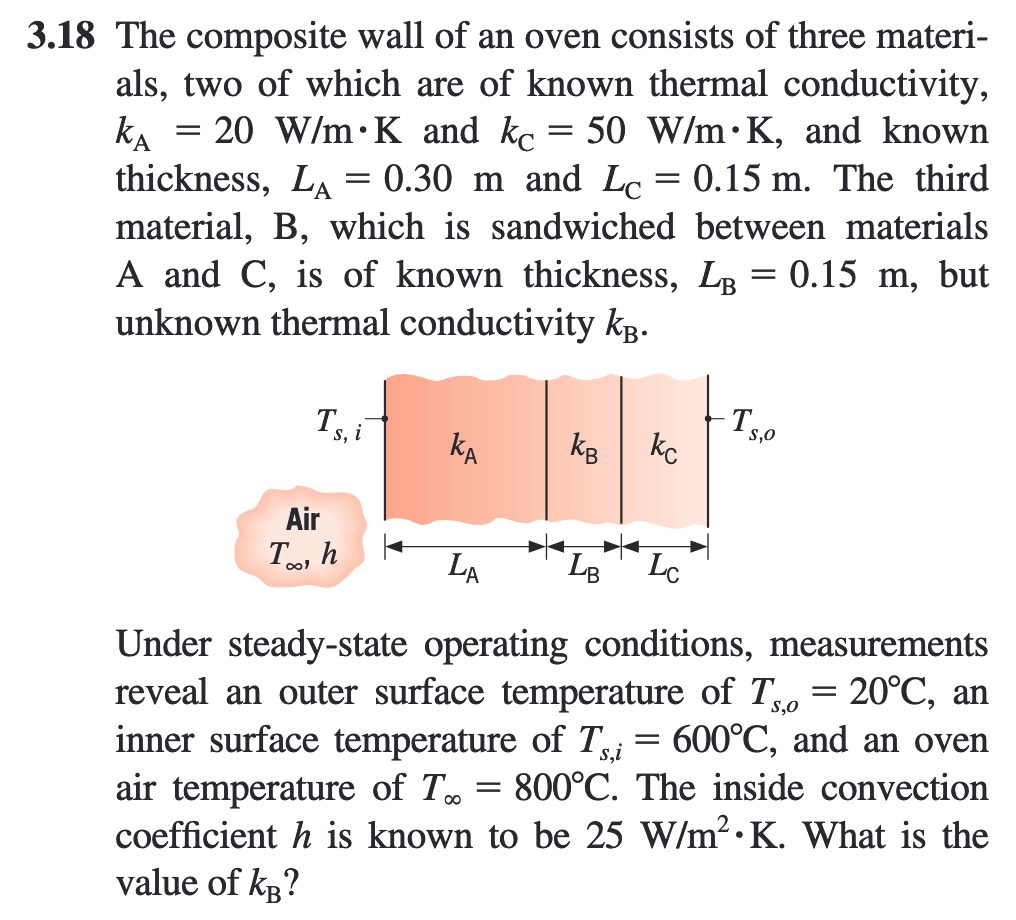
\includegraphics[width=.5\textwidth]{Figures/fig1.2.jpg}
    \end{figure}
\end{frame}

\begin{frame}{Problem 2 (3.18 in the book) Solution}
    \begin{columns}
        \column{.35\textwidth}
        \begin{figure}
            \centering
            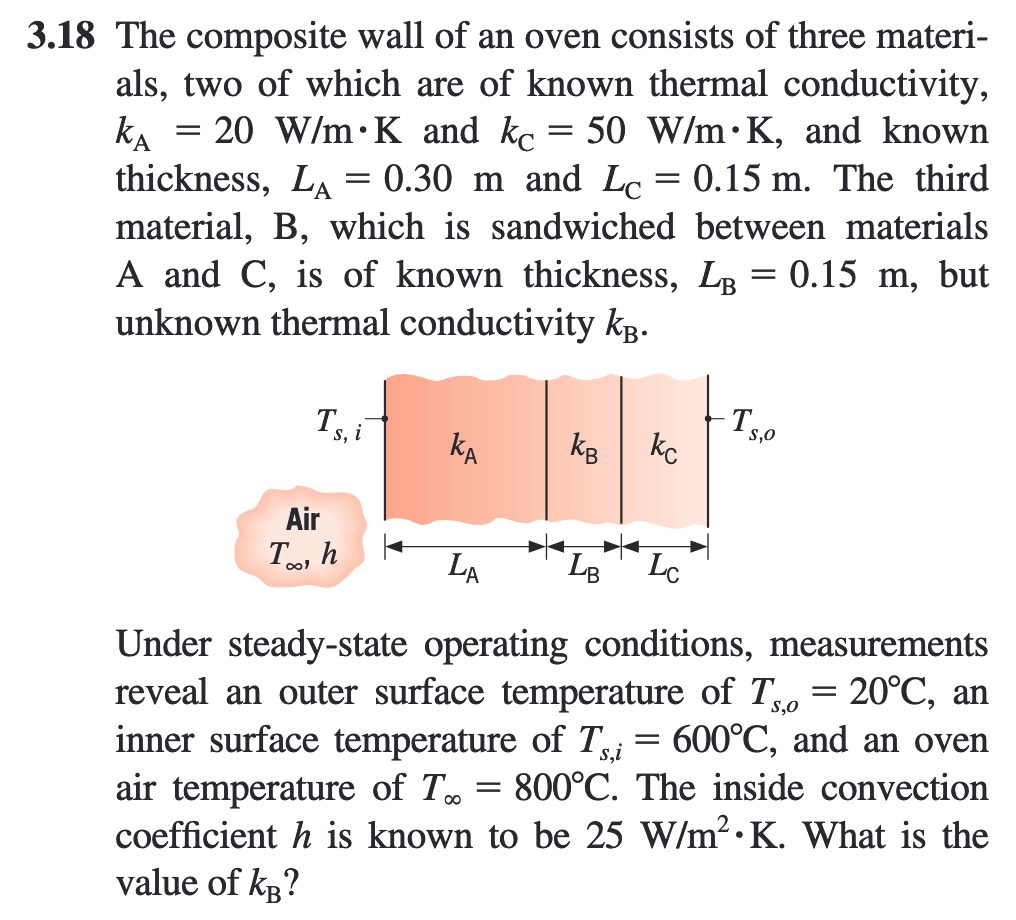
\includegraphics[width=\textwidth]{Figures/fig1.2.jpg}
        \end{figure}
        \column{.5\textwidth}
        \begin{figure}
            \centering
            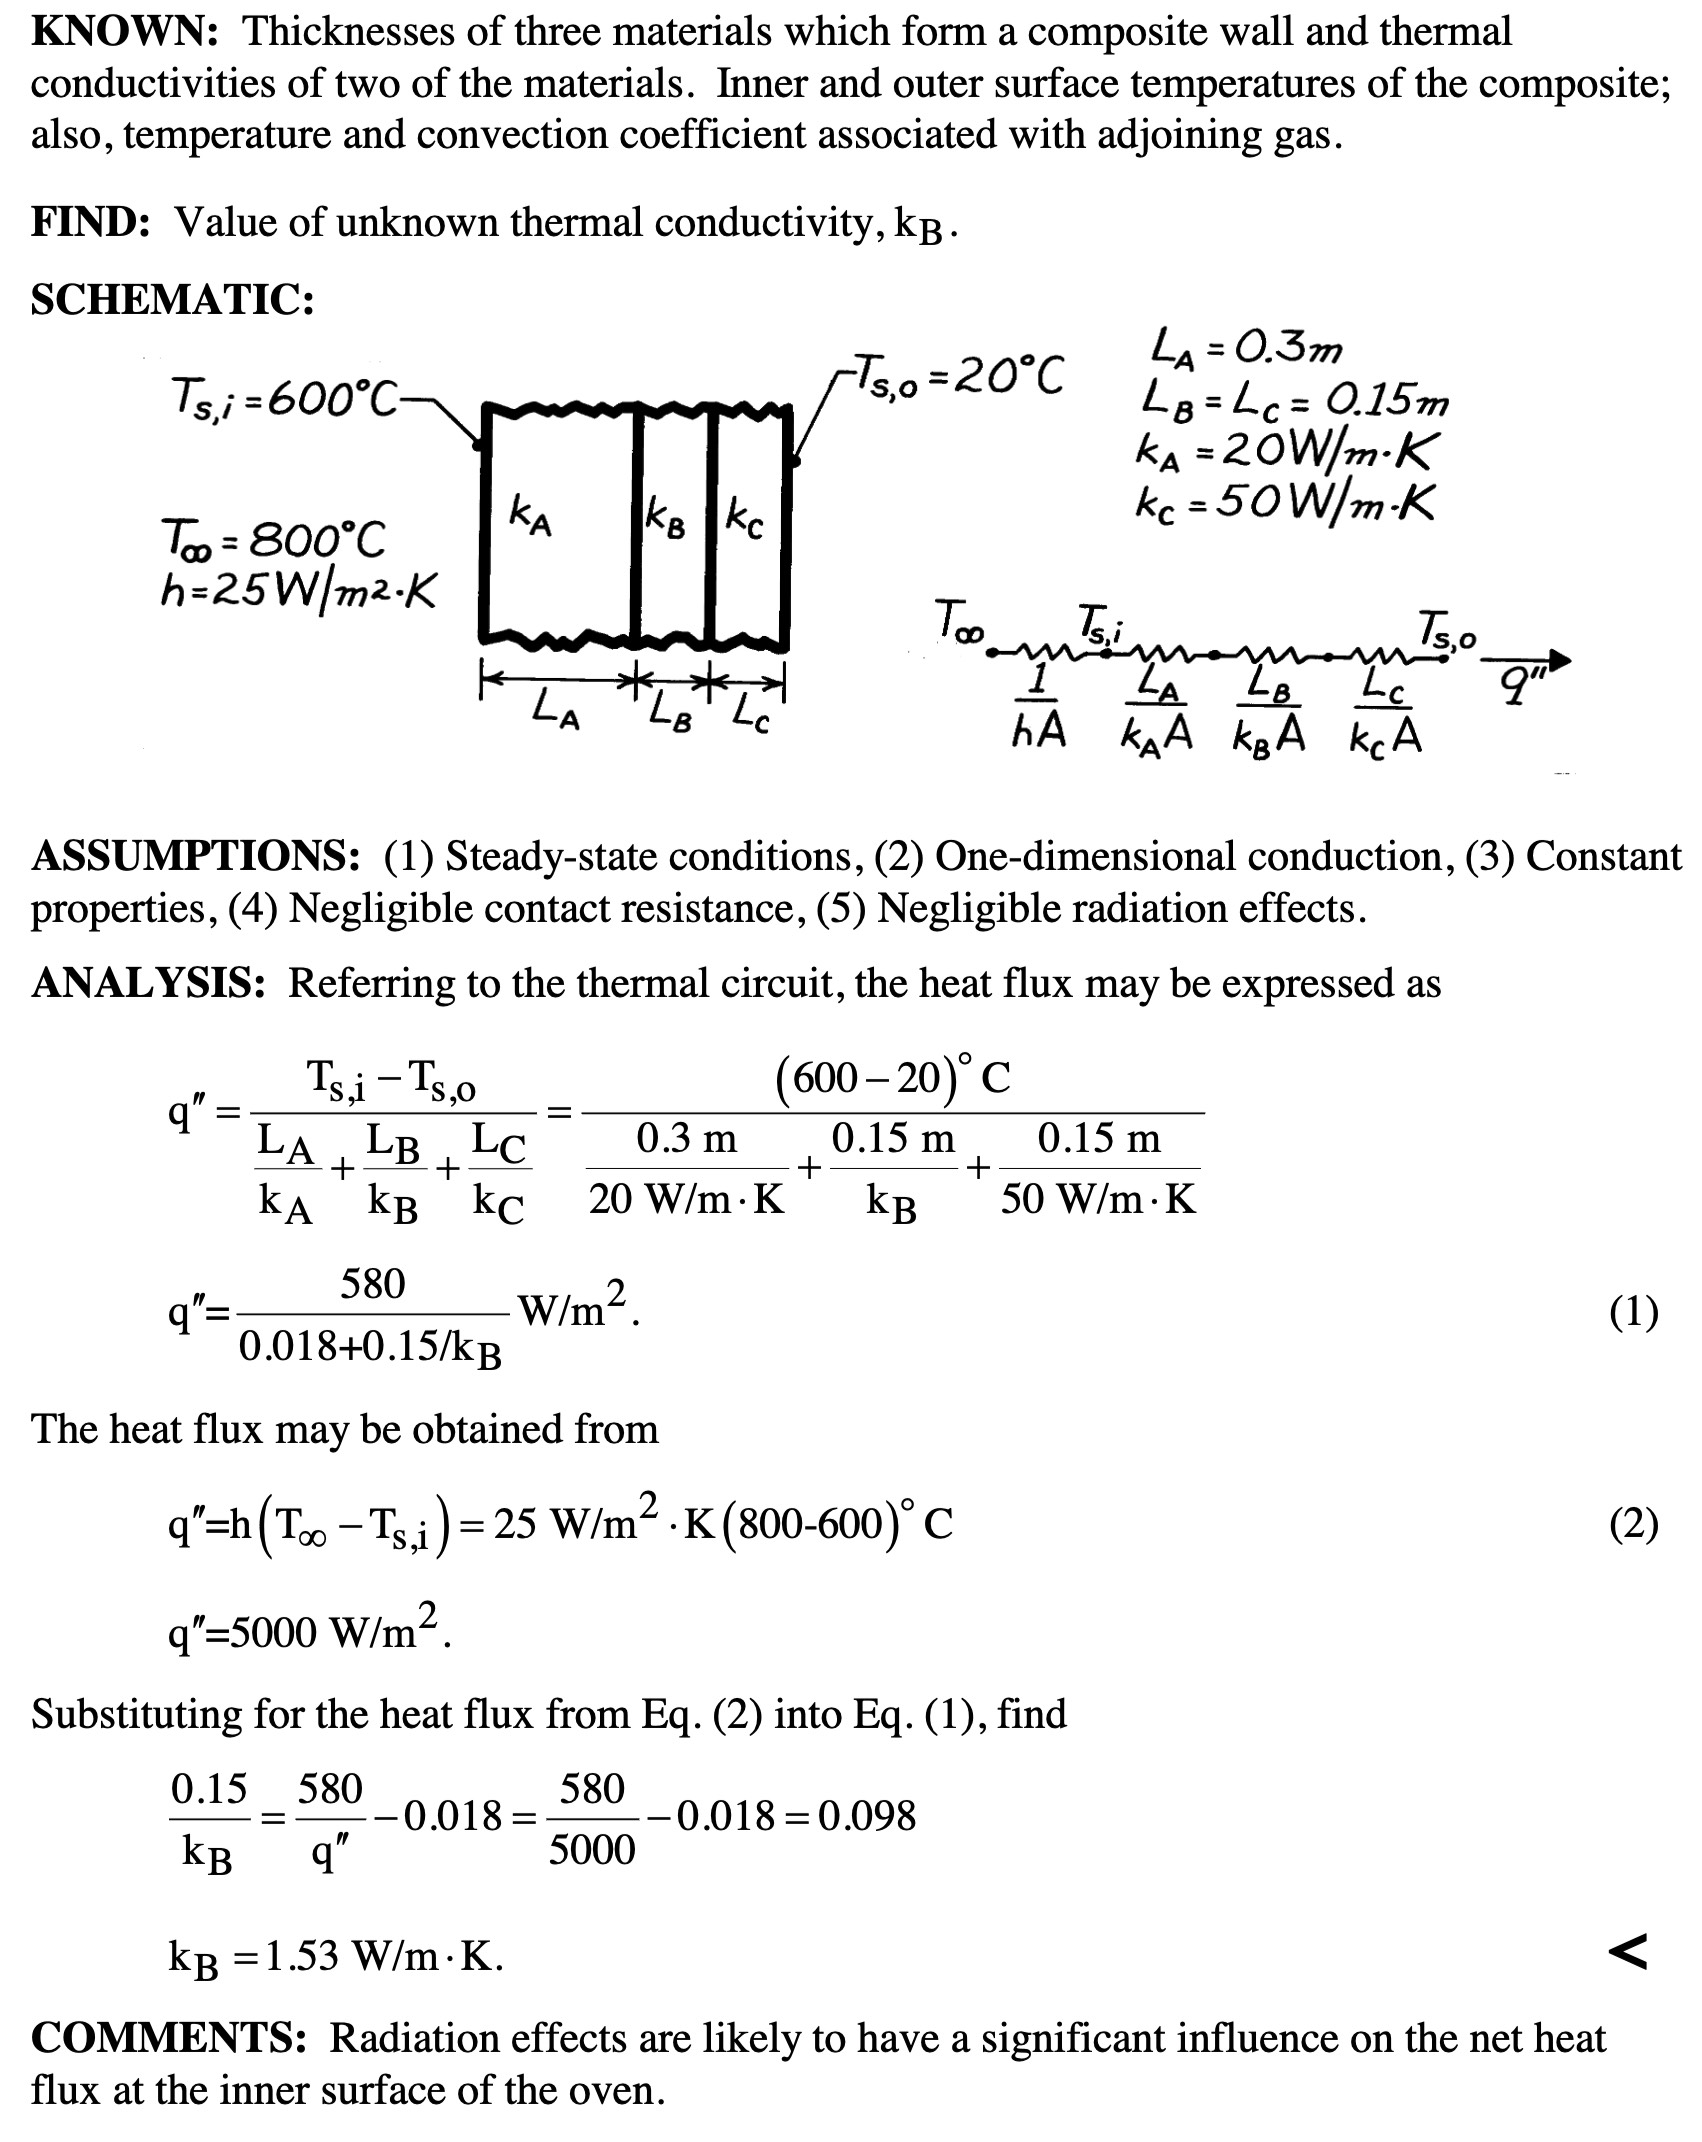
\includegraphics[width=.7\textwidth]{Figures/fig1.2_solution.jpg}
        \end{figure}
    \end{columns}
\end{frame}

\begin{frame}{Problem 3 (3.101 in the book)}
    \begin{figure}
        \centering
        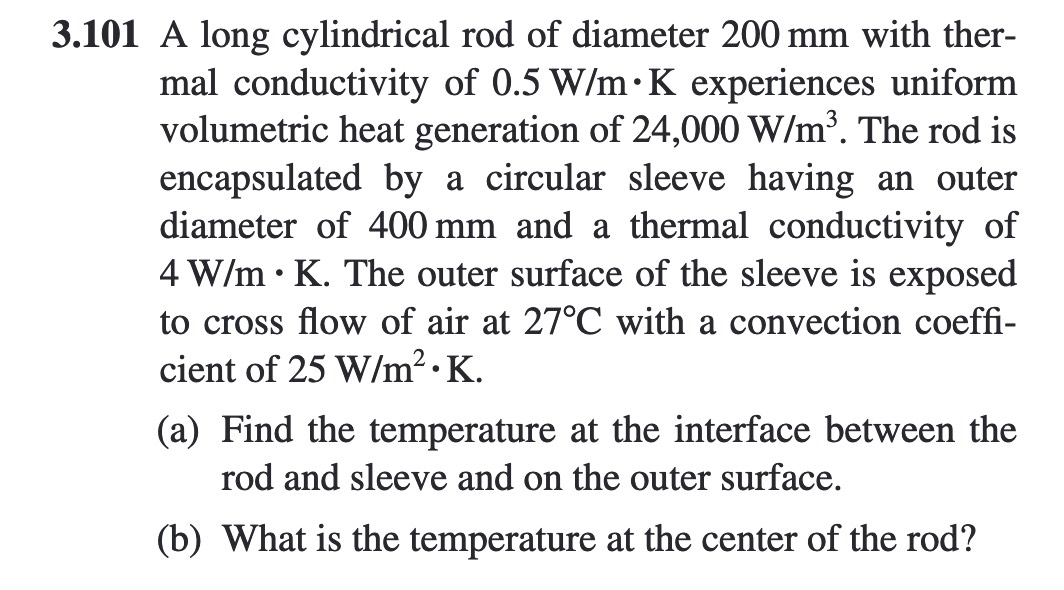
\includegraphics[width=.5\textwidth]{Figures/fig1.3.jpg}
    \end{figure}
    \myhl{Hint}:
    \begin{itemize}
        \item Thermal resistance of a cylinder with outer radius $r_2$ and inner radius $r_1$ is $R = \frac{1}{2\pi kL}\ln(r_2/r_1)$;
        \item Heat equation in cylindrical coordinates:
        \begin{equation}
            \frac{1}{r}\left(kr\frac{\partial T}{\partial r}\right) + \frac{1}{r^2} \frac{\partial }{\partial \Phi} \left(k\frac{\partial T}{\partial\Phi}\right) + \frac{\partial }{\partial z} \left(k\frac{\partial T}{\partial z}\right) + \dot{Q} = \rho c_p \frac{\partial T}{\partial t}
            \tag{2.26 in the book}
        \end{equation}
    \end{itemize}
\end{frame}

\begin{frame}{Problem 3 (3.101 in the book) Solution}
    \begin{columns}
        \column{.35\textwidth}
        \begin{figure}
            \centering
            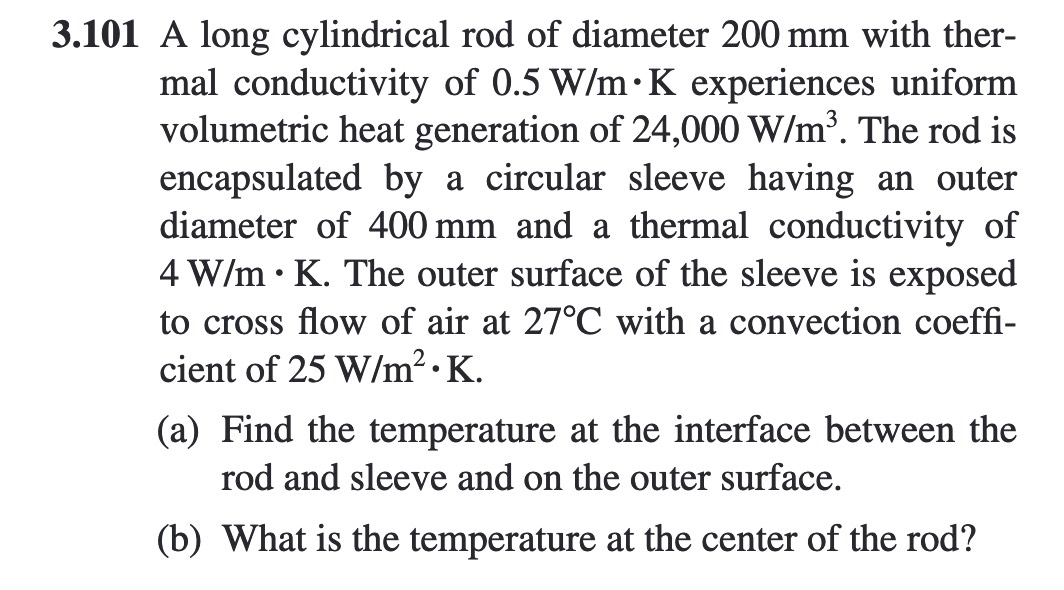
\includegraphics[width=\textwidth]{Figures/fig1.3.jpg}
        \end{figure}
        \column{.45\textwidth}
        \begin{figure}
            \centering
            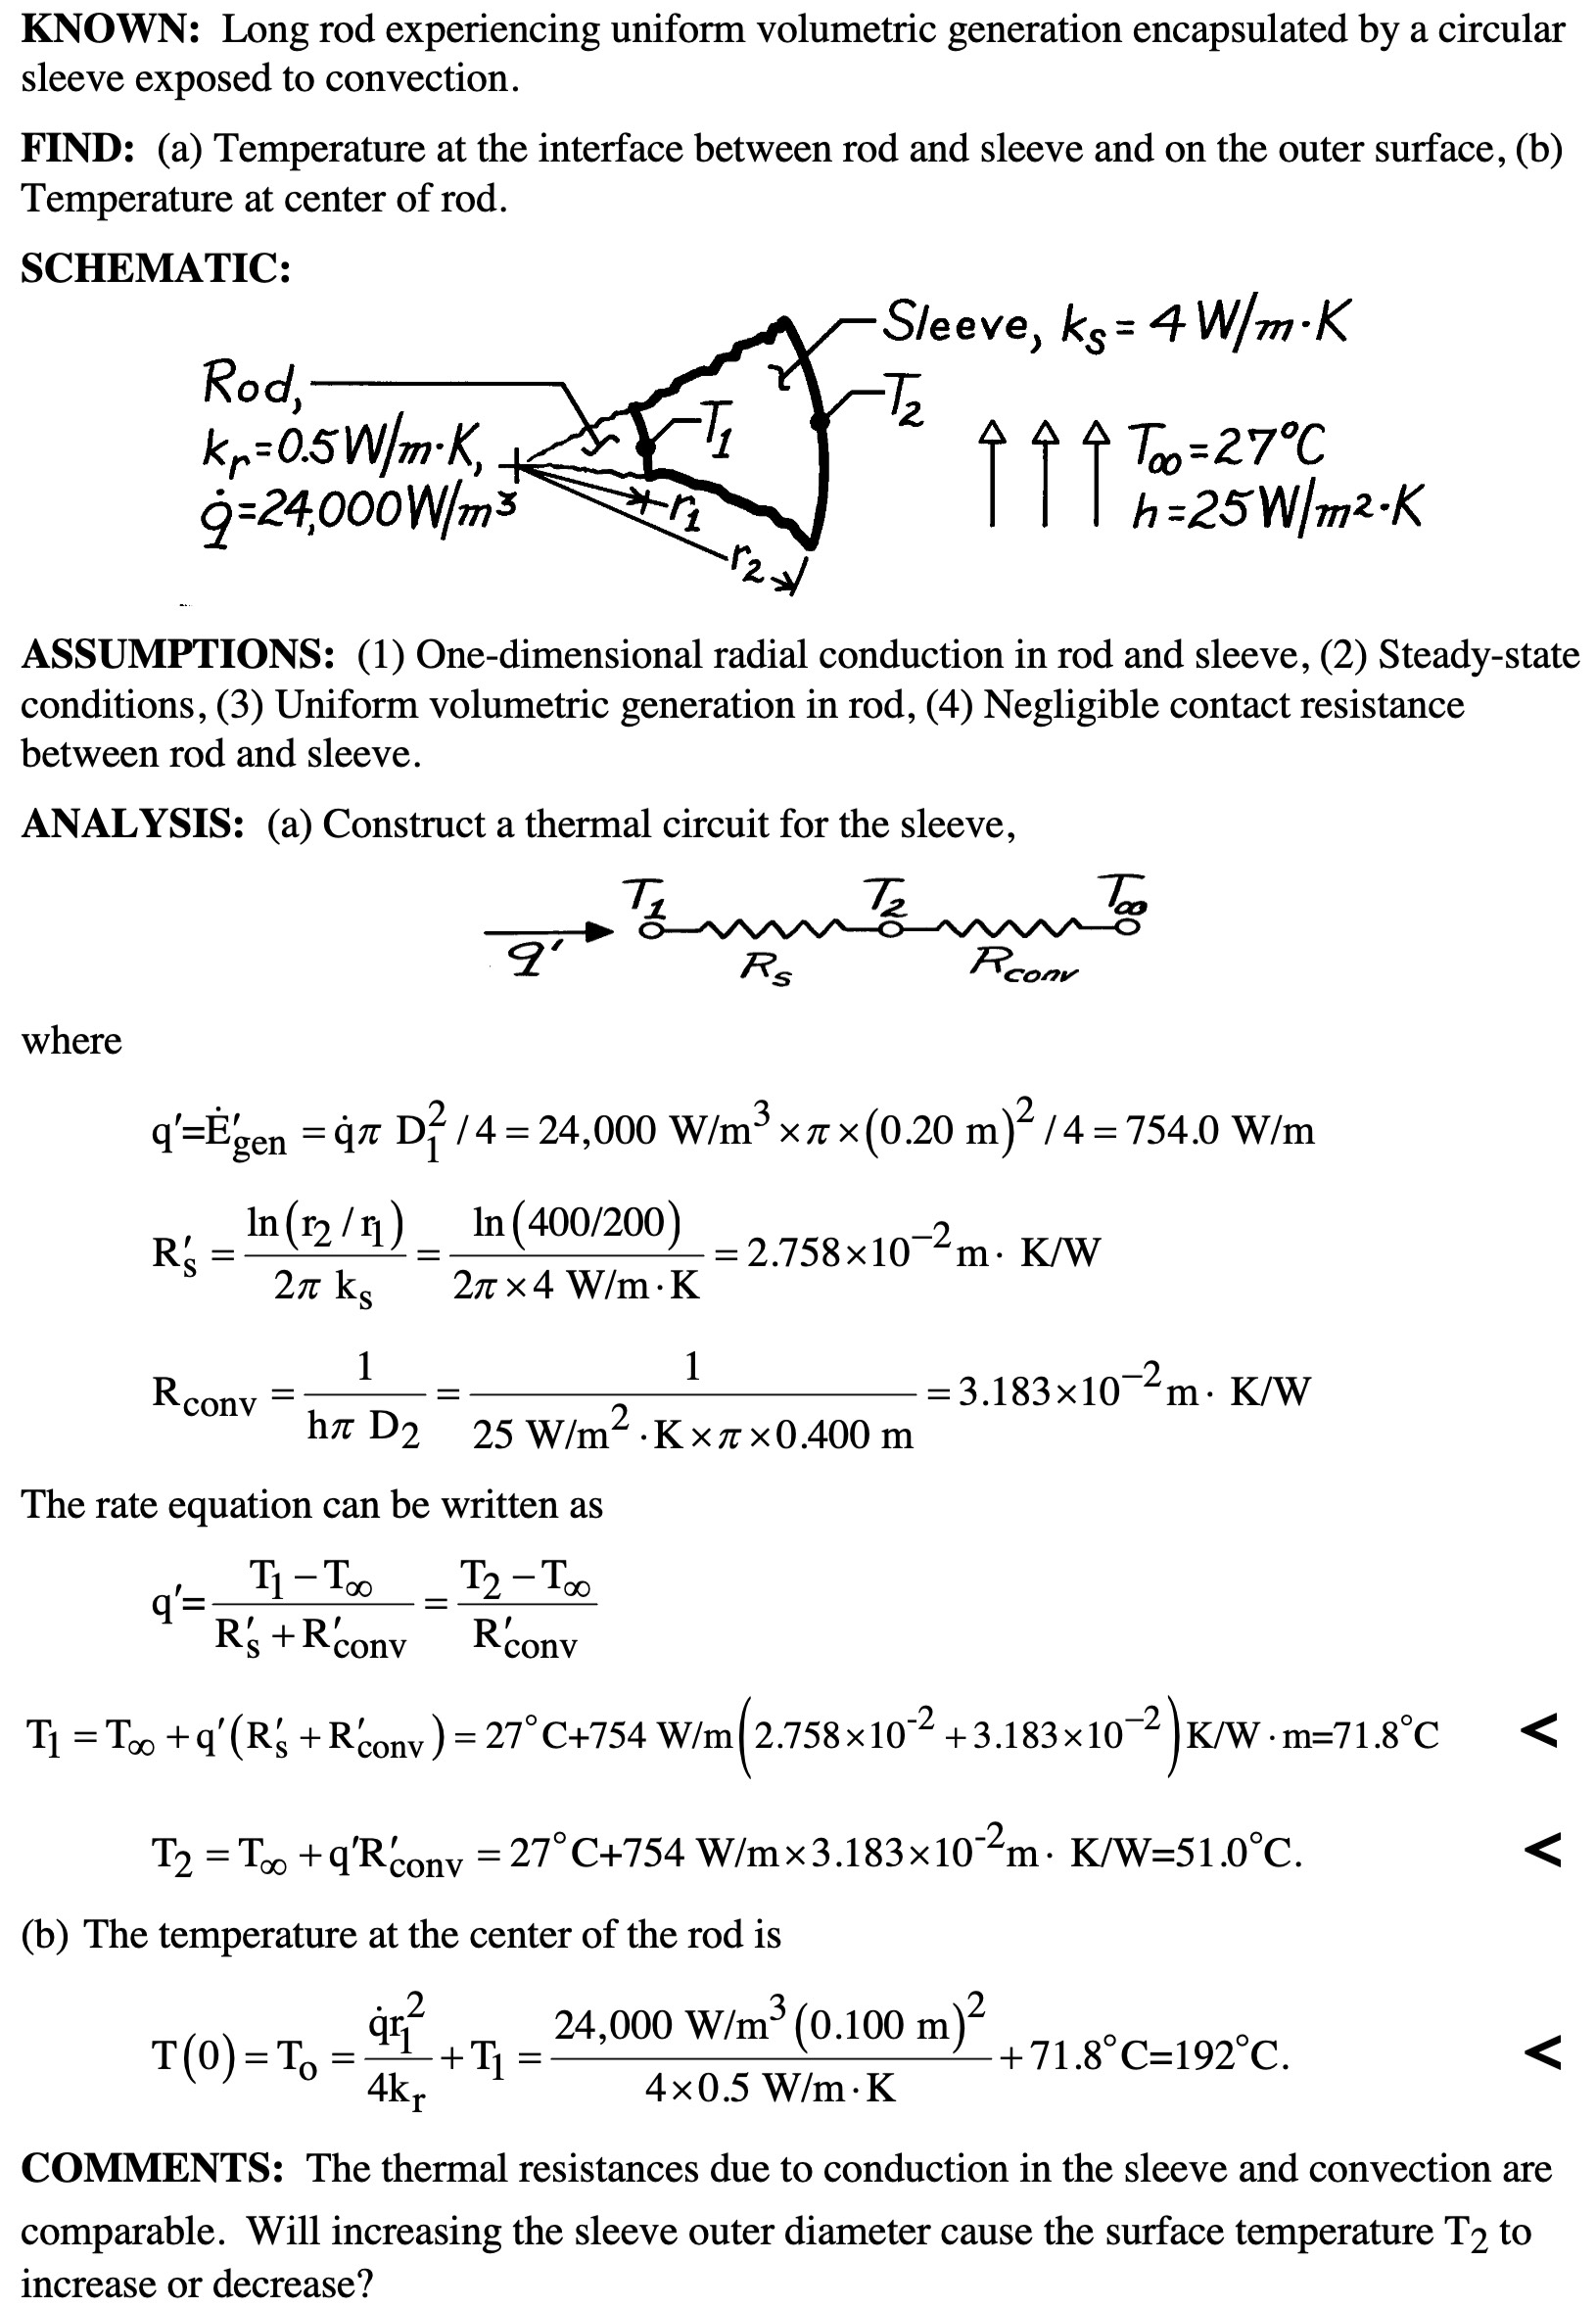
\includegraphics[width=.7\textwidth]{Figures/fig1.3_solution.jpg}
        \end{figure}
    \end{columns}
\end{frame}

\end{document}
